\documentclass[journal,10pt]{IEEEtai}
\usepackage{amsmath,amssymb,amsthm,bm}
\usepackage{booktabs,multirow,tabularx,array}
\usepackage{graphicx,subcaption}
\usepackage{algorithm}
\usepackage{algpseudocode}
\usepackage{xcolor}
\usepackage[hidelinks]{hyperref}
\usepackage[nameinlink,noabbrev]{cleveref}
\usepackage{url}
\newtheorem{proposition}{Proposition}
\newtheorem{assumption}{Assumption}
\newcommand{\method}{MiSFP}
\newcommand{\MissingResult}{\textemdash}
% Generated table rows (Sources/scripts/campaign/collect_misfp.py); primitive input works inside tabular.
\makeatletter\providecommand{\tabrows}[1]{\@@input #1 }\makeatother
\newcommand{\R}{\mathbb{R}}
\newcommand{\E}{\mathbb{E}}
\newcommand{\Wone}{W_1}
\newcommand{\todo}[1]{\textcolor{magenta}{[Draft: #1]}}
\title{MiSFP: Mixture-Preserving Prototyping for Hierarchical Split-Federated Learning}
\author{Dung T. Tran, Bumjin Jang, Van-Dinh Nguyen, and Kok-Seng Wong%
\thanks{Dung T. Tran is with Hanyang University ERICA, Ansan, Republic of Korea, and VinUniversity, Hanoi, Vietnam (e-mail: jacksontran@hanyang.ac.kr). Bumjin Jang is with Hanyang University ERICA, Ansan, Republic of Korea (e-mail: bjang@hanyang.ac.kr). Kok-Seng Wong is with VinUniversity, Hanoi, Vietnam (e-mail: ks.wong@vinuni.edu.vn). Corresponding author: Kok-Seng Wong. An earlier version of this paper was presented at the European Conference on Computer Vision (ECCV), 2026 \cite{tran2026h}.}
}
\begin{document}
\maketitle
\begin{abstract}
Hierarchical split federated learning distributes a network across clients, edge servers, and a cloud. H-SFP decouples training across tiers using synthetic features generated from class statistics, but a single diagonal Gaussian can obscure distinct feature clusters. We introduce \method{}, which communicates support-weighted mixtures of diagonal Gaussians with component caps and optional byte budgets at both split boundaries. Clients construct mixtures using fixed component requests or a validation-based selection heuristic. Receiving tiers retain components or compress them through deterministic same-class merging. After training its nonlinear segment, the edge re-estimates mixture statistics in its output space. We establish exact mass and diagonal-moment preservation, derive a per-merge transport bound, characterize packet and computational costs, and bound fixed-predictor loss discrepancies under explicit assumptions. Evaluation covers four classification datasets and ISIC-2018 segmentation, complemented by matched CIFAR-100 ablations. After 200 rounds, MiSFP-K4 achieves $\geq60\%$ accuracy on IID CIFAR-100, compared with $\geq55\%$ for H-SFP. Under Dirichlet partitioning with $\alpha=0.1$, it gains 3.97 percentage points with approximately 5.2\% more total communication and 92\% more prototype traffic. On ISIC-2018, it achieves $73.21\pm0.72\%$ IoU and $84.41\pm0.66\%$ Dice. Fidelity results remain metric-dependent, while shared-encoder controls demonstrate sensitivity to the extraction regime and its communication cost.
\end{abstract}

\begin{IEEEImpStatement}
This work examines statistical feature transfer for distributed learning with constrained device capacity and communication. Mixture-based class summaries offer a way to retain feature variation within and across clients, while component caps and optional packet budgets control representation size. The findings support evaluating prediction, representation fidelity, and encoder compatibility together, and reporting prototype traffic separately from model synchronization. Practical deployment requires further assessment of runtime overhead, performance under severe heterogeneity, and information exposure. Keeping raw examples local does not itself provide a formal privacy guarantee.
\end{IEEEImpStatement}

\begin{IEEEkeywords}
Federated learning, split learning, hierarchical learning, distributional prototypes, Gaussian mixtures, communication-constrained learning.
\end{IEEEkeywords}
\section{Introduction}
\label{sec:intro}

Federated learning (FL) enables distributed clients to train a shared model while keeping raw examples local~\cite{pmlr-v54-mcmahan17a}. Non-IID data and unequal local computation can cause client drift and objective inconsistency~\cite{li2020federated,10.5555/3495724.3496362}, while limited memory, processing capacity, and bandwidth restrict participation~\cite{MAL-083,9084352}. These challenges interact in hierarchical systems, where learning must accommodate distributed data and resources.

Hierarchical FL (HierFL) organizes communication through edge aggregators~\cite{9148862,9488756,rana2022hierarchical}, while split learning (SL) distributes network computation across devices and servers~\cite{GUPTA20181,vepakomma2019split}. SplitFed and HierFL methods combine partitioned execution with federated synchronization~\cite{thapa2022splitfed,quan2023hiersfl,10980018}. Conventional split execution exchanges intermediate activations and backward gradients, coupling successive segments during optimization. H-SFP uses a statistical interface: class means and diagonal standard deviations define Gaussian summaries from which upper tiers synthesize training features, enabling training without cross-tier backpropagation~\cite{tran2026h}.

The effectiveness of this interface depends on the structure retained by each class summary. A class can contain multiple feature clusters within one client or across client subpopulations (Fig.~\ref{fig:illustration}(a,b)). Collapsing separated clusters into one Gaussian can allocate density to regions between them, even when class means and coordinate-wise variances are preserved (Fig.~\ref{fig:illustration}(c)). A full covariance captures correlations at quadratic storage cost, but a single Gaussian remains unimodal. Multiple diagonal components offer several centers while keeping per-component moment storage linear in feature dimension.

\begin{figure*}[t]
\centering
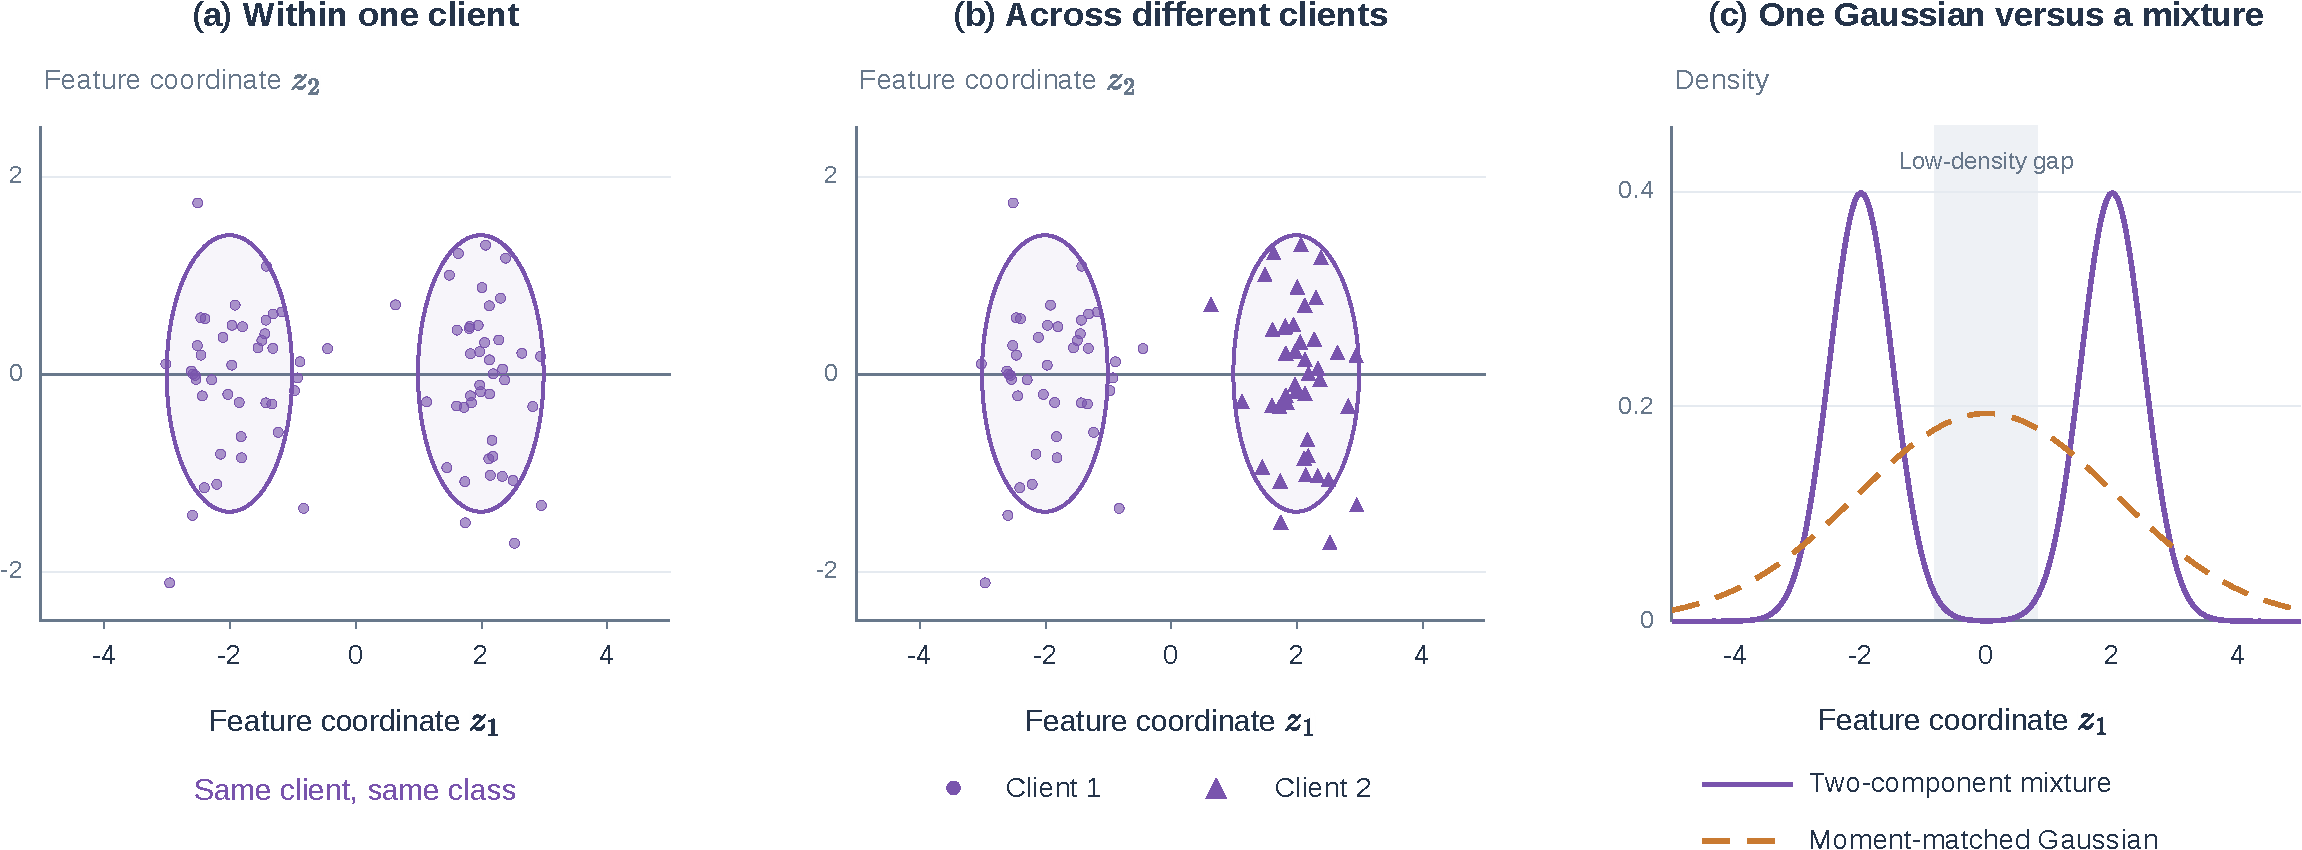
\includegraphics[width=\linewidth]{figures/misfp_multimodality.pdf}
\caption{Illustration of within-class multimodality: (a) modes within one client and (b) modes contributed by different clients. (c) First-coordinate marginal densities of a two-component mixture and its moment-matched single Gaussian. In this example, moment matching preserves the class mean and coordinate-wise variances but allocates more density between the modes.}
\label{fig:illustration}
\end{figure*}

Prototype learning, distillation, and generation establish the value of transferring compact class information and synthetic features~\cite{tan2022fedproto,lin2020ensemble,zhu2021data}. CCVR and FedImpro reconstruct feature distributions for classifier calibration or high-level training~\cite{luo2021ccvr,tang2024fedimpro}. FedPFT transfers parametric distributions from frozen foundation-model embeddings for one-shot classifier training~\cite{beitollahi2025fedpft}, while FedGMKD uses Gaussian mixtures to derive prototype features and soft predictions~\cite{zhang2024fedgmkd}. These provide foundations for distribution-based learning. Hierarchical split training additionally requires repeated transformation and compression as successive, spatially distributed model parts.

Three considerations govern this process. First, local class support constrains which components can be estimated reliably, while communication capacity limits their retention. Second, the nonlinear edge segment changes the feature distribution, requiring statistics to be re-estimated in its output space. Third, independently updated model segments can produce apparent separation through coordinate mismatch as well as population variation. Component allocation must therefore be considered jointly with support weighting, boundary transformation, coordinate compatibility, and packet cost.

We introduce \method{}, a hierarchical split-training framework that communicates support-weighted mixtures of diagonal Gaussians. Clients construct mixtures using fixed component requests or a validation-based selection heuristic. Receiving tiers retain same-class components and use deterministic greedy merges when compression is required. The edge trains from mixture samples and re-estimates output-space statistics before transmission to the cloud. Component caps and optional serialized-byte budgets control retention separately at the client--edge and edge--cloud boundaries. Gradients remain within each tier, while total communication includes periodic model synchronization.
The main contributions are:
\begin{enumerate}
    \item A support-weighted mixture interface for representing multiple class-conditional components and generating upper-tier training features in a hierarchical split model.

    \item A construction and compression procedure combining fixed or validation-selected local component counts, nonlinear-boundary re-estimation, and deterministic same-class merging under component caps and optional boundary-specific byte budgets.

    \item An analysis establishing exact mass and diagonal-moment preservation, bounding the transport discrepancy introduced by an individual merge, and characterizing packet costs, computational complexity, and fixed-predictor loss discrepancies under explicit assumptions.

    \item An evaluation combining classification and segmentation benchmarks with ablations of component retention, packet budgets, representation fidelity, encoder compatibility, and communication and resource costs.
\end{enumerate}
\section{Related Work}
\label{sec:related}
\begin{table*}[t]
\caption{Comparison of representative prototype and feature-distribution transfer methods. The representation column summarizes information used for transfer; additional model-parameter exchange may occur.}
\label{tab:extension}
\centering
\small
\setlength{\tabcolsep}{4pt}
\begin{tabularx}{\textwidth}{@{}p{2.05cm}XXp{2.55cm}@{}}
\toprule
Method & Class or feature representation & Main role in training & Organization\\
\midrule
FedProto~\cite{tan2022fedproto} & Class-mean prototypes & Regularization of local representations & Client--server\\
FedGen~\cite{zhu2021data} & Learned class-conditional feature generator & Synthetic features guide local training & Client--server\\
CCVR~\cite{luo2021ccvr} & Gaussian feature-distribution estimates & Virtual features recalibrate the classifier after federated training & Client--server; post-training calibration\\
FedImpro~\cite{tang2024fedimpro} & Shared Gaussian feature statistics & Reconstructed features augment high-level local training & Iterative client--server\\
FedPFT~\cite{beitollahi2025fedpft} & Parametric feature distributions, including Gaussian mixtures & Synthetic-feature classifier training with frozen feature extractors & One-shot federation\\
FedGMKD~\cite{zhang2024fedgmkd} & Mixture-derived prototype features and soft predictions & Knowledge alignment and discrepancy-aware aggregation & Iterative client--server\\
H-SFP~\cite{tran2026h} & Class means and diagonal standard deviations; one Gaussian per class & Synthetic inputs train successive upper-tier segments & Client--edge--cloud\\
MiSFP & Support-weighted mixtures of diagonal Gaussians & Mixture synthesis, output-space re-estimation, and moment-preserving compression & Client--edge--cloud; optional boundary byte budgets\\
\bottomrule
\end{tabularx}
\end{table*}
\subsection{Federated and Hierarchical Split Learning}

FedAvg combines local optimization with weighted parameter aggregation~\cite{pmlr-v54-mcmahan17a}. FedProx, FedNova, and SCAFFOLD address heterogeneous local training through proximal regularization, update normalization, and control variates, respectively~\cite{li2020federated,10.5555/3495724.3496362,pmlr-v119-karimireddy20a}. Device capacity and communication remain important constraints~\cite{MAL-083,9084352}. HeteroFL and selective-kernel approaches accommodate weaker clients by adapting the computation assigned to them~\cite{diao2021heterofl,niu2023overcoming}.

HierFL organizes aggregation across clients, edges, and the cloud~\cite{9148862,9488756,rana2022hierarchical}. SL partitions network computation between devices and servers~\cite{GUPTA20181,vepakomma2019split}; SplitFed and hierarchical split-learning methods combine partitioned execution with federated synchronization~\cite{thapa2022splitfed,quan2023hiersfl,10980018}. Conventional split execution exchanges activations and corresponding gradients, with communication-efficient variants reducing their payload and storage costs~\cite{11091500,zhang2025amperecommunicationefficienthighaccuracysplit}. H-SFP instead communicates class means and diagonal standard deviations to synthesize training inputs for successive segments, keeping gradients within each tier~\cite{tran2026h}. MiSFP examines how multiple components can be retained and compressed within this form of statistical interface.

\subsection{Prototype and Feature-Distribution Transfer}

FedProto exchanges class-mean prototypes to regularize local representations~\cite{tan2022fedproto}, while subsequent methods refine prototype alignment and personalization under non-IID data~\cite{10660707,bensiah2025feddpa}. Representation-sharing methods distinguish common features from personalized prediction components~\cite{collins2021exploiting}. Knowledge-transfer approaches provide complementary signals: FedDF uses ensemble distillation~\cite{lin2020ensemble}, FedGen learns a class-conditional feature generator~\cite{zhu2021data}, and MOON uses model-level contrastive learning~\cite{9578660}. Contrastive and supervised contrastive objectives provide broader foundations for representation learning~\cite{chen2020simple,khosla2020supervised}.

Several methods directly reconstruct feature distributions. CCVR recalibrates a federated classifier after training using virtual representations sampled from estimated Gaussian models~\cite{luo2021ccvr}. FedImpro separates low-level and high-level model components and uses shared, reconstructed feature distributions to augment high-level local training~\cite{tang2024fedimpro}. These establish that synthetic features derived from communicated statistics can support both classifier calibration and ongoing FL training.

Mixture-based transfer provides a particularly close comparison. FedPFT fits parametric distributions, including Gaussian mixtures, to frozen foundation-model embeddings and transfers their parameters for one-shot synthetic-feature classifier training~\cite{beitollahi2025fedpft}. FedGMKD uses mixture-derived prototype features and soft predictions for knowledge alignment and discrepancy-aware aggregation~\cite{zhang2024fedgmkd}. MiSFP studies repeated distribution transfer through spatially distributed client, edge, and cloud segments, where the intermediate nonlinear transformation requires output-space re-estimation.

\subsection{Mixture Representation and Compression}

Gaussian mixtures are an established representation for distributions with multiple components~\cite{mclachlan2000finite}. Pairwise moment-matching reduction replaces components with fewer Gaussian summaries; KL-based reduction uses an upper bound to guide pair selection~\cite{runnalls2007kl}. Moment pooling and greedy component reduction therefore have substantial prior foundations.

Optimal transport provides tools for comparing probability distributions and Gaussian components~\cite{villani2009optimal}. Wasserstein-type mixture distances also use restricted couplings to obtain tractable transport formulations between Gaussian mixtures~\cite{delon2020wasserstein}. A distance between individual components, a transport bound, and the exact distance between complete mixtures are distinct quantities. MiSFP uses a support-weighted diagonal-Gaussian pair score and analyzes its local effect without claiming globally optimal mixture reduction.

MiSFP coordinates mixture construction, support weighting, nonlinear-boundary re-estimation, and class-preserving compression across two split boundaries. Locally updated encoders make coordinate compatibility relevant, while component caps and optional serialized-byte budgets constrain retention. Its contribution concerns this repeated statistical interface for synthetic upper-tier training. \Cref{tab:extension} summarizes the distinctions.

\section{System Model and Problem Formulation}
\label{sec:problem}

We consider a three-tier system comprising clients, edge servers, and a cloud server. Client $i\in\mathcal C_e$ is assigned to edge $e\in\mathcal E$ and holds $\mathcal D_i=\{(x_j,y_j)\}$. The network comprises a client encoder $u_{\theta_i}$, an edge segment $h_{\theta_e}$, and a cloud head $g_{\theta_g}$, yielding $f_{i,e}=g_{\theta_g}\circ h_{\theta_e}\circ u_{\theta_i}$. Raw examples and per-example annotations remain local; communicated summaries contain class identifiers and aggregate feature statistics. Upper-tier segments train on synthetic features without backpropagation across split boundaries.

At round $t$, individual feature vectors at the client--edge and edge--cloud boundaries belong to $\mathcal Z_{ce}\subseteq\R^{d_{ce}}$ and $\mathcal Z_{ec}\subseteq\R^{d_{ec}}$, respectively. For classification, $z=u_{\theta_i^t}(x)$ is an image embedding and $s=h_{\theta_e^t}(z)$ is its edge-output representation. For segmentation, the encoder retains a spatial map, with $z_p=[u_{\theta_i^t}(x)]_p$ at location $p$. The upper-tier mappings operate pointwise, with $s_p=h_{\theta_e^t}(z_p)$. The same statistical interface therefore supports image embeddings and labeled spatial embeddings, as detailed in \cref{sec:method}.

For each class $c$ represented by valid features at client $i$, let $P_{ic}$ denote its client--edge feature distribution at the current round. Round indices are omitted from distributions and mixture parameters for readability. MiSFP approximates $P_{ic}$ using a support-weighted mixture of diagonal Gaussians:
\begin{equation}
\label{eq:mixture}
\begin{aligned}
Q_{ic}
&=
\sum_{r=1}^{R_{ic}}
\pi_{icr}\mathcal N
\bigl(\bm\mu_{icr},\mathrm{diag}(\bm v_{icr})\bigr),\\
\pi_{icr}
&=
\frac{n_{icr}}{n_{ic}},
\qquad
n_{ic}=\sum_{r=1}^{R_{ic}}n_{icr}.
\end{aligned}
\end{equation}
Here, $R_{ic}$ is the component count, $n_{icr}>0$ is the empirical number of valid features assigned to component $r$, and $\bm\mu_{icr}$ and $\bm v_{icr}$ are its mean and unfloored population diagonal variance. Support counts image embeddings for classification and labeled spatial embeddings for segmentation.

Edge--cloud summaries use the same mixture form in $\mathcal Z_{ec}$. Their component masses carry incoming class support and may become noninteger effective estimates after output-space refitting. These masses are distinct from the Monte Carlo sample counts used to estimate output statistics. Component probabilities remain support-weighted, whereas the upper-tier class sampling prior is uniform over represented classes.

Pooling requires consistent class labels and compatible feature definitions. Each packet records its split boundary, feature dimension and shape, extraction regime, and model version. Compatible metadata establishes structural consistency, but independently updated model segments may still express features in different coordinates. Source separation can therefore reflect both population structure and coordinate mismatch. Mixture moments and distributional discrepancies are defined in the raw, unnormalized space at each boundary. Relating discrepancies across boundaries requires accounting for the intervening map $h_{\theta_e}$.

When byte budgets are enabled, $B_{ce}$ and $B_{ec}$ limit the complete serialized sizes of outgoing client and edge packets, including metadata and component statistics. Component caps provide additional retention constraints. Compression retains at least one component for every represented class; if the minimum class-preserving packet exceeds its budget, infeasibility is reported. Model-synchronization traffic is accounted for separately and included in total training communication.

The design problem is to allocate and compress class-conditional components that support prediction while satisfying the configured retention and communication constraints. This requires balancing representation fidelity, available class support, and packet cost. \Cref{tab:notation} summarizes the notation.

\begin{table}[t]
\caption{Principal notation used throughout the paper.}
\label{tab:notation}
\centering
\small
\begin{tabularx}{\columnwidth}{@{}lX@{}}
\toprule
Symbol & Meaning\\
\midrule
$t$ & Communication round\\
$i,e,c,r$ & Client, edge, class, and component indices\\
$\mathcal C_e,\mathcal E$ & Clients assigned to edge $e$ and set of edge servers\\
$u,h,g$ & Client encoder, edge segment, and cloud head\\
$\mathcal Z_{ce},\mathcal Z_{ec}$ & Boundary feature spaces of dimensions $d_{ce},d_{ec}$\\
$P,Q$ & Target and represented class-conditional distributions\\
$n_{icr},\pi_{icr}$ & Component support mass and within-class weight\\
$\bm\mu,\bm v$ & Mean and unfloored population diagonal variance\\
$R_{ic},R_c$ & Local and pooled retained component counts for class $c$\\
$N_c$ & Total class support mass in a pooled mixture\\
$K_{\max}$ & Maximum candidate local component count\\
$M_c,M_c^{\mathrm{bd}}$ & Per-class synthetic training and boundary-estimation sample counts\\
$B_{ce},B_{ec}$ & Optional serialized-packet budgets at the two boundaries\\
\bottomrule
\end{tabularx}
\end{table}
\begin{figure*}[h!]
\centering
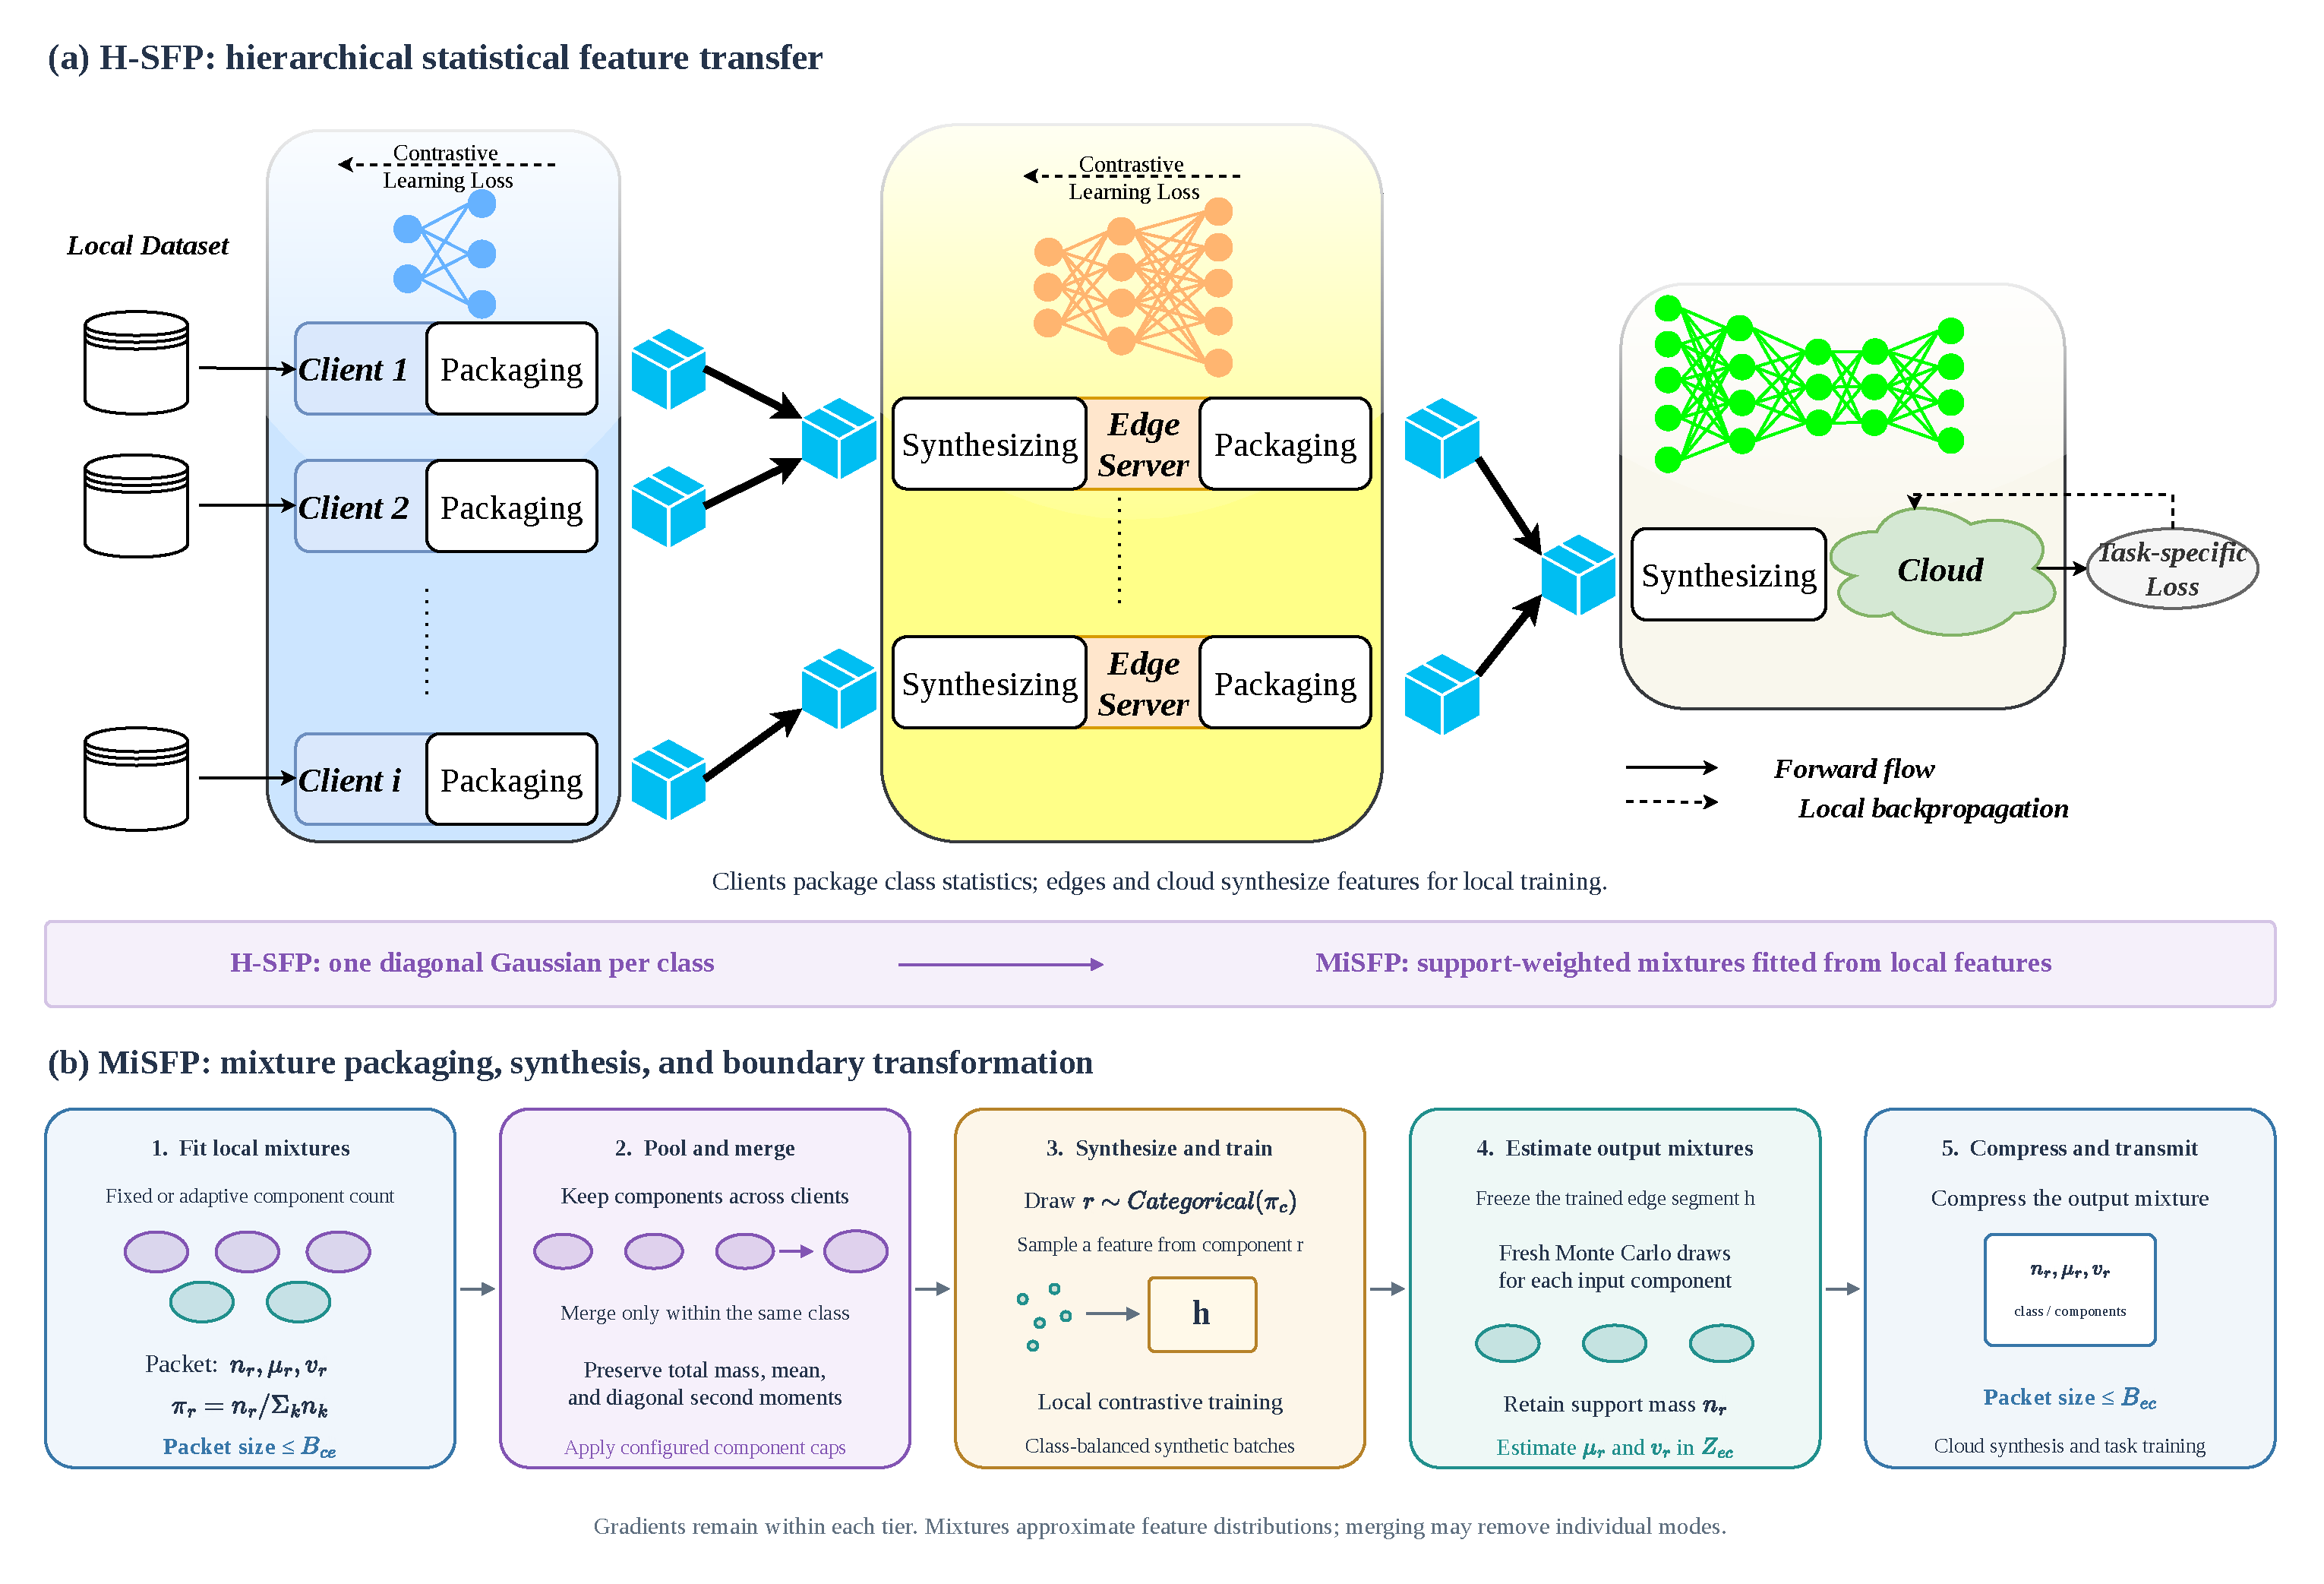
\includegraphics[width=\textwidth]
{figures/misfp_architecture.pdf}
\caption{Statistical feature transfer across clients,
edges, and the cloud.
(a) H-SFP~\cite{tran2026h} generates upper-tier training
inputs from single-Gaussian class summaries.
Solid arrows indicate forward flow; dashed arrows
indicate local backpropagation.
(b) MiSFP constructs and compresses mixtures, trains
the edge from synthetic features, re-estimates
output-space statistics, and compresses the outgoing
packet for cloud training.
Step~4 illustrates the default \emph{propagate} mode,
which retains incoming component support masses.}
\label{fig:architecture}
\end{figure*}
\section{MiSFP}
\label{sec:method}

H-SFP trains successive model segments from synthetic
features generated using single-Gaussian class
summaries~\cite{tran2026h}.
MiSFP uses support-weighted mixtures to retain multiple
components within and across clients.
Its execution comprises local mixture construction,
class-wise pooling and compression, synthetic edge
training, output-space re-estimation, and cloud training
(Fig.~\ref{fig:architecture}).
Gradients remain within the segment being optimized;
parameter synchronization is performed separately.

\subsection{Local Training and Mixture Construction}

Mixture statistics are estimated in the raw,
unnormalized feature spaces defined in
\cref{sec:problem}.
Contrastive similarities and cloud prediction use
the stabilized normalization
\begin{equation}
\label{eq:normalization}
\operatorname{norm}_{\epsilon_n}(\bm r)
=
\frac{\bm r}{\max\{\|\bm r\|_2,\epsilon_n\}},
\qquad \epsilon_n>0.
\end{equation}
The normalization floor is fixed, and the cloud applies
the same normalization during training and inference.
Communicated moments are computed before normalization.

Client $i$ trains its encoder using supervised
contrastive learning~\cite{khosla2020supervised}.
Let $\mathcal A$ index a batch and define
$\bm q_a=\operatorname{norm}_{\epsilon_n}(\bm r_a)$
for raw representation $\bm r_a$.
The positive set is
$\mathcal P(a)=
\{p\in\mathcal A\setminus\{a\}:y_p=y_a\}$,
and $\mathcal A_+$ contains the anchors with
nonempty positive sets.
The objective is
\begin{equation}
\label{eq:supervised_contrastive}
\begin{aligned}
\mathcal L_{\mathrm{SC}}
&=
-\frac{1}{|\mathcal A_+|}
\sum_{a\in\mathcal A_+}
\frac{1}{|\mathcal P(a)|}
\sum_{p\in\mathcal P(a)}
\log\rho_{ap},\\
\rho_{ap}
&=
\frac{\exp(\bm q_a^\top\bm q_p/\tau)}
{\sum_{b\in\mathcal A\setminus\{a\}}
 \exp(\bm q_a^\top\bm q_b/\tau)},
\end{aligned}
\end{equation}
with $\tau=0.1$.
Classification batches contain two augmented views
of each image.
Anchors without positives are excluded, and an update
is skipped if no valid anchors remain.

After local training, the encoder is fixed for feature
extraction.
Nonfinite feature vectors are discarded and counted.
Classification uses embeddings after encoder pooling;
segmentation uses labeled spatial embeddings
(Section~\ref{subsec:segmentation}).

For each represented class, seeded k-means++
initialization and Lloyd iterations determine
component centers.
Center fitting may use a reservoir of at most
4096 features.
Assignment counts and population moments nevertheless
use every valid feature in the corresponding fitting set.
Each component stores a support mass and two
length-$d$ moment vectors, giving
$\mathcal O(Kd)$ parameter storage for $K$ components.
Although each component has diagonal covariance,
differences between component means allow the mixture
to exhibit cross-coordinate dependence.

Fixed variants request $K\in\{1,2,4\}$ components.
For $K>1$, every component must satisfy the configured
minimum support, whose default is $s_{\min}=3$.
If this condition fails, fitting is repeated with
a smaller $K$.
A nonempty class can fall back to one component even
when its total support is below $s_{\min}$.
Thus, this support condition constrains multi-component
fitting; it does not suppress small nonempty classes.

Adaptive construction selects $K$ for each
client--class pair.
For classification, a seeded split reserves 30\%
of valid class features for validation.
Client-side segmentation uses image-disjoint subsets.
Let $\mathcal V_{ic}$ denote the validation features
and $q_{ic}^{(K)}$ a candidate density fitted without
using those features.
Feasible candidates are scored by
\begin{equation}
\label{eq:component_selection}
\begin{aligned}
\mathcal J_{ic}(K)
&=
-\frac{1}{d_{ce}|\mathcal V_{ic}|}
\sum_{z\in\mathcal V_{ic}}
\log q_{ic}^{(K)}(z)+\lambda(K-1),
\end{aligned}
\end{equation}
for $K\in\{1,\ldots,K_{\max}\}$.
Likelihood evaluation uses a positive variance floor.
The default configuration uses $K_{\max}=4$,
$\lambda=0$, and at least four validation features.
A minimizing candidate with $K>1$ is accepted only if
$
\mathcal J_{ic}(1)-\mathcal J_{ic}(K)>\delta,
$
where $\delta=0.02$ nat/dimension by default.
When a positive penalty is configured, the required
unpenalized NLL improvement is
$\delta+\lambda(K-1)$.
Insufficient validation data or support yields $K=1$.
The selected mixture is refitted on all valid class
features, with support checks applied again.

This selector is a local density-fit heuristic;
it does not directly optimize the receiving model's
predictive loss.
Fixed and adaptive allocations are therefore evaluated
as separate configurations in \cref{sec:experiments}.
Table~\ref{tab:variants} distinguishes local component
requests from hierarchical retention.
Experiment-specific overrides are reported with
the evaluation settings.

\begin{table}[t]
\caption{Default MiSFP component requests and per-class
retention limits.
Support checks can reduce the local request.
For the non-K1 variants, the regular edge-input cap
is unset and a safety cap of 32 is configured.
``--'' denotes no explicit cap.
Optional byte budgets can further reduce retention.}
\label{tab:variants}
\centering
\small
\setlength{\tabcolsep}{4pt}
\begin{tabularx}{\columnwidth}{@{}Xcccc@{}}
\toprule
Variant
& Local
& Edge
& Edge
& Cloud\\
& $K$
& input
& output
& pool\\
\midrule
K1       & $1$    & $1$  & $1$ & $1$\\
Edge     & $1$    & $32$ & $4$ & --\\
K2       & $2$    & $32$ & $4$ & --\\
K4       & $4$    & $32$ & $4$ & --\\
Adaptive & $\leq4$ & $32$ & $4$ & --\\
\bottomrule
\end{tabularx}
\end{table}

\begin{algorithm}[t]
\caption{Client packet construction}
\label{alg:client}
\begin{algorithmic}[1]
\Require features by class, selection settings,
         $s_{\min}$, optional budget $B_{ce}$
\For{each locally represented class $c$}
    \State discard and count nonfinite features;
           skip the class if none remain
    \State select $K$ using the fixed request or
           \eqref{eq:component_selection}
    \State refit on all valid class features;
           reduce $K>1$ if support checks fail
    \State compute
           $(n_{icr},\bm\mu_{icr},\bm v_{icr})$
           from all final assignments
\EndFor
\State apply same-class compression under $B_{ce}$
       if configured
\State serialize the packet; report infeasibility
       if the budget cannot be met
\end{algorithmic}
\end{algorithm}
\subsection{Pooling and Budgeted Merging}

A receiving tier concatenates compatible components
separately by class
(Fig.~\ref{fig:architecture}(b), Step~2).
Pooling and pair comparisons are performed within
one boundary feature space, subject to the compatibility
checks in \cref{sec:problem}.
Local component indices do not identify corresponding
modes across sources.

For two same-class components with positive masses
$a$ and $b$, the pooled parameters are
\begin{align}
m
&=a+b,
\qquad
\bm\mu=
\frac{a\bm\mu_a+b\bm\mu_b}{m},
\label{eq:poolmean}\\
\bm v
&=
\frac{a}{m}
\left[\bm v_a+(\bm\mu_a-\bm\mu)^2\right] +
\frac{b}{m}
\left[\bm v_b+(\bm\mu_b-\bm\mu)^2\right].
\label{eq:poolvar}
\end{align}
Squares are elementwise.
These expressions preserve the total mass, mean,
and coordinate-wise second moments of the represented
components in exact arithmetic
(\cref{sec:analysis}).

Candidate pairs are scored by
\begin{equation}
\label{eq:mergecost}
\Delta(a,b)
=
\frac{ab}{a+b}
\left(
\|\bm\mu_a-\bm\mu_b\|_2^2
+
\|\sqrt{\bm v_a}-\sqrt{\bm v_b}\|_2^2
\right).
\end{equation}
The parenthesized term is the squared
$2$-Wasserstein distance between the two diagonal
Gaussians.
The support factor incorporates their masses into
the pair ranking.
This does not equal the distance between
the mixtures before and after merging.

Compression first enforces the configured per-class
caps by repeatedly merging the admissible pair with
the smallest $\Delta$.
If an outgoing packet still exceeds its byte budget,
additional same-class merges minimize $\Delta$
divided by the positive reduction in complete
serialized size.
For fixed-size component records and an unchanged
header, each merge saves the same number of bytes,
so this ranking reduces to the ranking by $\Delta$.
Canonical component ordering resolves ties
deterministically.

The optional budgets $B_{ce}$ and $B_{ec}$ apply
to outgoing client and edge packets, including metadata.
Receiver-side pools are governed separately by their
component caps.
At least one component remains for every represented
class.
If the minimum class-preserving packet exceeds the
budget, compression reports infeasibility under the
configured warning or error policy. Feasibility is determined from the serialized packet size.
The procedure provides deterministic component reduction
under the configured constraints.
Its moment identities do not guarantee optimal compression.
Figure~\ref{fig:merging} shows the process.

\begin{figure}[t]
\centering
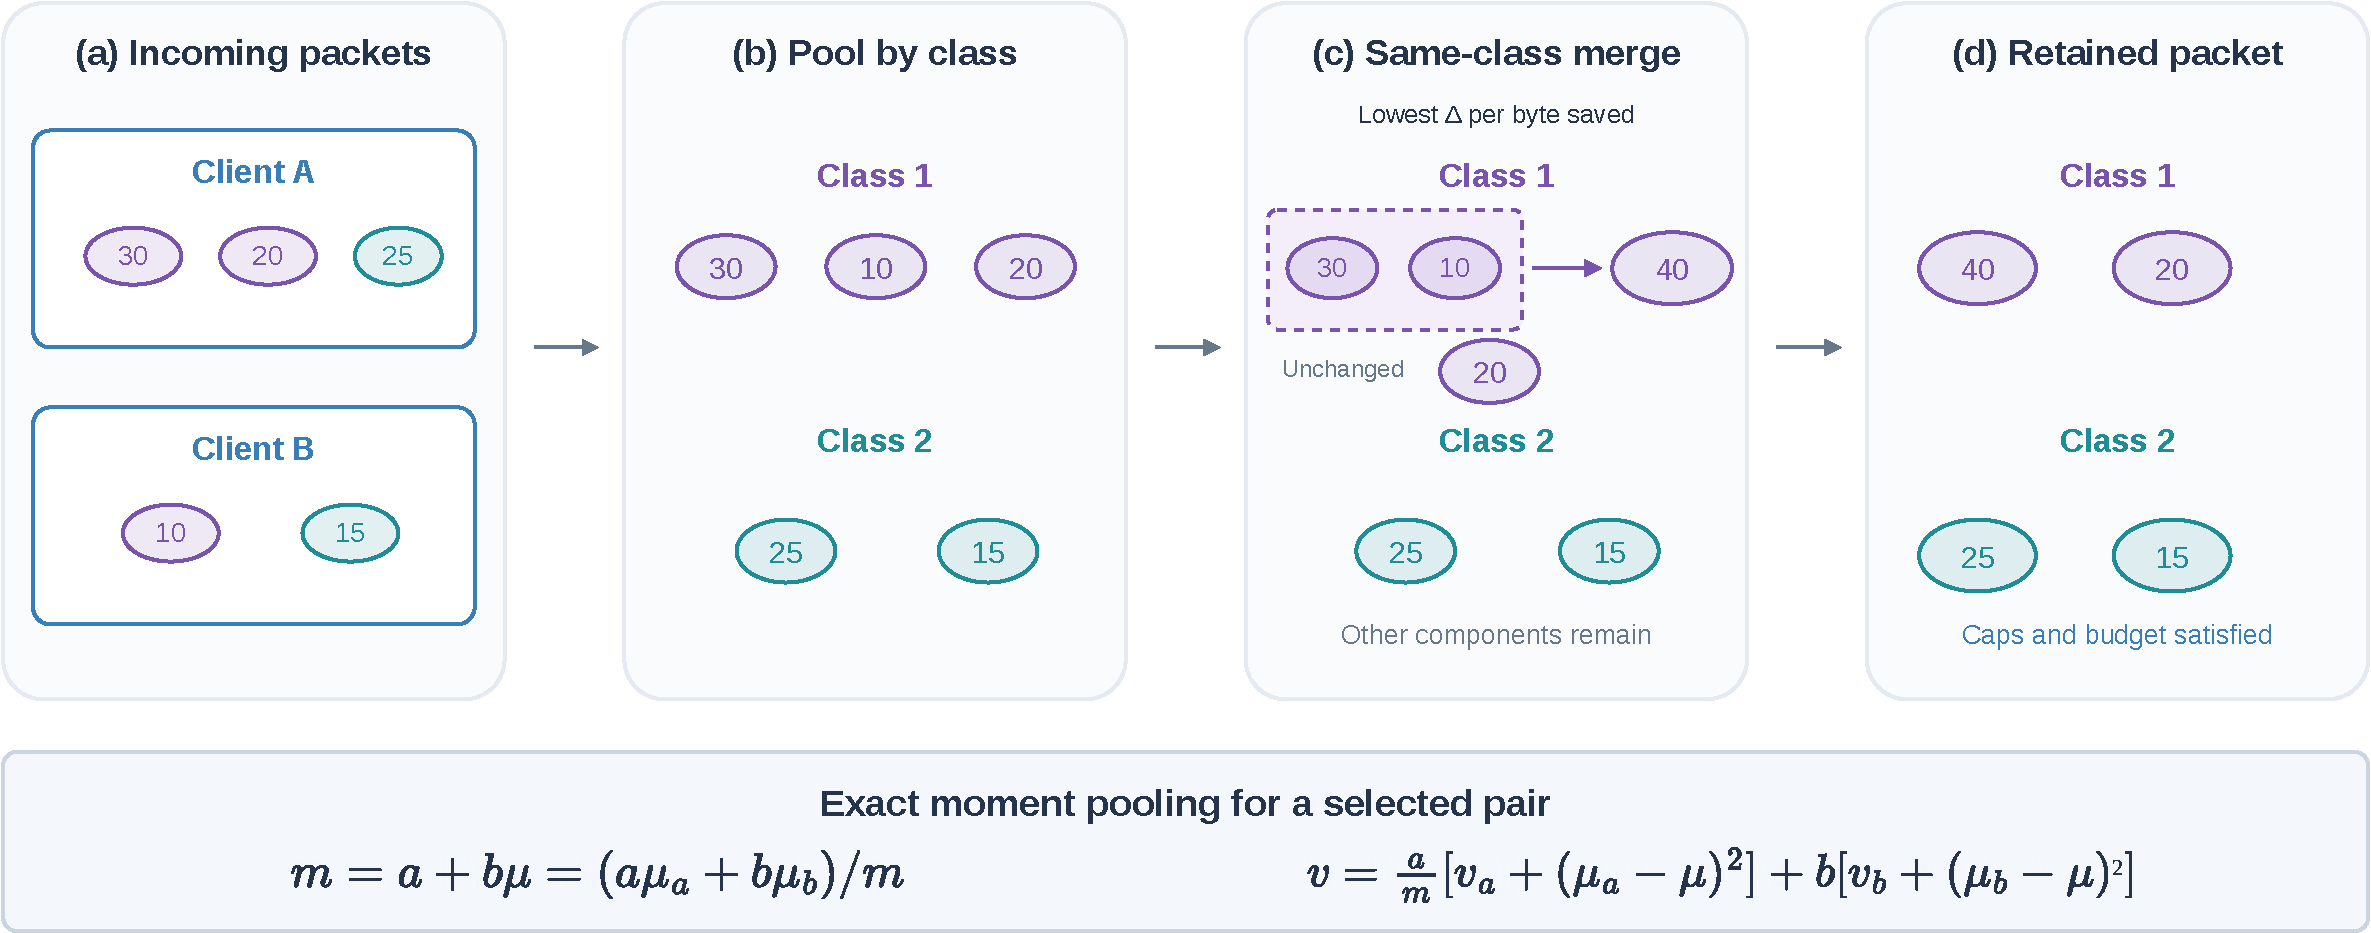
\includegraphics[width=\columnwidth]
{figures/misfp_merging.pdf}
\caption{Class-preserving pooling and compression.
Colors denote classes and numbers denote component
support masses.
Same-class merges preserve aggregate mass, means,
and coordinate-wise second moments in exact arithmetic.
The $\Delta$-per-byte criterion applies during
byte-budget compression.}
\label{fig:merging}
\end{figure}

\subsection{Synthesis and Nonlinear Boundary Transformation}

For a retained class mixture $Q_c$, let $\bm\pi_c$
contain its normalized component masses.
MiSFP first draws
$r\sim\mathrm{Categorical}(\bm\pi_c)$
and then generates
\begin{equation}
\label{eq:mixture_sampling}
\tilde z
=
\bm\mu_{cr}
+
\sqrt{\max(\bm v_{cr},\epsilon_s)}
\odot\bm\xi,
\qquad
\bm\xi\sim\mathcal N(\bm 0,I),
\end{equation}
where $\epsilon_s>0$, and the maximum and square root
are elementwise.
A balanced synthesis schedule supplies $M_c$ features
per represented class, while within-class sampling
follows the support weights.
Stored variances remain unfloored during construction
and merging; floors are applied only during
likelihood evaluation and sampling.

The edge trains $h_{\theta_e}$ from raw synthetic
inputs using \eqref{eq:supervised_contrastive}
on normalized edge outputs.
Each selected class contributes at least two synthetic
features per batch.
The received mixture statistics remain fixed
during this optimization.

After training, the edge fixes $h_{\theta_e}$
and estimates summaries in its raw output space.
A nonlinear map generally transforms a Gaussian
into a non-Gaussian distribution.
Consequently, the input parameters cannot simply
be reused in $\mathcal Z_{ec}$.
MiSFP supports two finite-sample estimation modes.

In the default \emph{propagate} mode
(Fig.~\ref{fig:architecture}(b), Step~4),
the edge draws a fixed number of fresh Monte Carlo
samples from each retained input component,
using 50 samples per component by default.
The transformed samples determine one output mean
and population diagonal variance per input component.
Each output retains its incoming support mass.
Equal sampling effort therefore does not make
the mixture weights uniform.

In \emph{refit} mode, the edge draws
$M_c^{\mathrm{bd}}$ fresh features from the complete
class mixture and transforms them through $h_{\theta_e}$.
This boundary-estimation count is configured separately
from the training sample count and defaults to
200 features per class.
The outputs are reclustered using the configured
output-component selection rule.
Each output component receives its assignment fraction
multiplied by the incoming class support, yielding
a potentially noninteger effective mass.

Both modes approximate the transformed sampling
distribution.
The output components are compressed under
the edge-output cap and optional $B_{ec}$.
Algorithm~\ref{alg:edge} shows the operation.

\begin{algorithm}[t]
\caption{Edge receive--train--emit operation}
\label{alg:edge}
\begin{algorithmic}[1]
\Require compatible client packets, component caps,
         optional budget $B_{ec}$, estimation mode
         and sample counts
\State concatenate received components by class
\State apply configured caps to the pooled input
\State sample class-balanced features using
       \eqref{eq:mixture_sampling}
\State train $h_{\theta_e}$ using
       \eqref{eq:supervised_contrastive}, then fix it
\If{mode is \emph{propagate}}
    \For{each retained input component}
        \State draw and transform the configured
               number of fresh Monte Carlo samples
        \State estimate output moments;
               retain the incoming support mass
    \EndFor
\Else
    \State draw and transform
           $M_c^{\mathrm{bd}}$ features per class
    \State refit output mixtures; assign effective
           masses from assignment fractions
           and incoming class support
\EndIf
\State compress under the output cap and optional $B_{ec}$
\State serialize the packet; report infeasibility
       if the budget cannot be met
\end{algorithmic}
\end{algorithm}

\subsection{Cloud Training and Model Synchronization}
\label{subsec:training}

The cloud pools compatible edge-output components
by class, applies any configured component cap,
and synthesizes a class-balanced training set
in $\mathcal Z_{ec}$.
The head $g_{\theta_g}$ applies
\eqref{eq:normalization} followed by a linear classifier
and is trained using cross entropy,
$
\ell_{\theta_g}(s,c)
=
-\log[\operatorname{softmax}(g_{\theta_g}(s))]_c
$.
The same normalization is applied to real features
during inference.
Morover, parameter synchronization follows two intervals.
Every $t_1$ rounds, each edge averages the latest
encoder update from every client that participated
during the preceding window.
Each client contributes once, weighted by its
training-dataset size.
The resulting encoder is broadcast to all attached
clients; an edge without updates retains its
previous checkpoint.
Every $t_2$ rounds, the cloud separately averages
edge-level encoder checkpoints and edge-segment
parameters, weighting edge $e$ proportionally to
$N_e=\sum_{i\in\mathcal C_e}|\mathcal D_i|$.
The aggregated encoder and edge segment are broadcast
through the hierarchy, while the cloud head remains
central.
The synchronization schedule uses $t_1=5$
and $t_2=10$.

Synchronization follows the round's training updates.
Within-edge aggregation precedes global aggregation
when both are due.
Subsequent packets identify their extraction model version, although periodic synchronization does not ensure coordinate alignment between locally updated encoders.
Total communication includes mixture packets and
parameter exchanges.
Matched H-SFP and MiSFP comparisons use the same
training objectives, task architectures, and
synchronization schedule.
MiSFP-K1 remains a separate control because it uses
the mixture packet path and moment-pooling operator.

\subsection{Application to Semantic Segmentation}
\label{subsec:segmentation}

For segmentation, the client retains the 128-channel
spatial feature map produced by ResNet-18 through
layer~2.
Ground-truth masks are resized to this grid using
nearest-neighbor interpolation.
Valid spatial embeddings are grouped by pixel label to construct foreground and background mixtures.
Component support counts the embeddings assigned to each one. Additionally, the edge applies a $1\times1$ convolution from 128 to 256 channels followed by ReLU, and the cloud uses a pointwise two-class head.
The client encodes spatial context; the upper-tier
mappings operate on individual embeddings.
Normalization in \eqref{eq:normalization} is applied
across channels at each location, allowing these
mappings to train on synthesized
features.

Client training applies~\eqref{eq:supervised_contrastive} to labeled spatial embeddings~\cite{wang2021pixelcontrast}.
Geometric augmentations are applied consistently to images and masks. Adaptive client construction uses image-disjoint fitting and validation subsets, followed by a final refit using all eligible local training features.
Aggregation is weighted by counts, separately from pixel-component masses.

Edge and cloud training use the synthetic-feature procedure above, with contrastive and pixelwise cross-entropy objectives, respectively.
During inference, the model preserves
the spatial feature grid.
Two-class logits are bilinearly upsampled to the
original image resolution before classwise argmax.
Foreground IoU and Dice are evaluated on complete
predicted masks.
\section{Analysis}
\label{sec:analysis}

We analyze moment preservation, the distributional change caused by an individual merge, packet and computational costs, and the sensitivity of a fixed predictor to feature-distribution approximation.

\begin{proposition}[Exact pooled diagonal moments]
\label{prop:moments}
Let $a,b\geq0$ with $m=a+b>0$, and let the components have finite means and finite, nonnegative population diagonal variances. In exact arithmetic, the merge defined by \cref{eq:poolmean,eq:poolvar} preserves total mass, the first moment, and coordinate-wise second moments. Consequently, any finite sequence of same-class merges preserves the class mass, mean, and coordinate-wise second moments of the unmerged mixture.
\end{proposition}

\begin{proof}
The merged mass is $m=a+b$, and $m\bm\mu=a\bm\mu_a+b\bm\mu_b$. For coordinate $j$, substituting \cref{eq:poolvar} and using $m\mu_j=a\mu_{a,j}+b\mu_{b,j}$ gives
$
m(v_j+\mu_j^2)
=
a(v_{a,j}+\mu_{a,j}^2)
+
b(v_{b,j}+\mu_{b,j}^2).
$
Each merge therefore preserves the unnormalized first and coordinate-wise second moments. Repeated application establishes the class-level result.
\end{proof}

These identities concern the represented mixture with unfloored variances in exact arithmetic. They do not imply preservation of its density, modes, or full covariance. Rounding, serialization, and sampling floors introduce additional discrepancies. The next proposition relates the merge score to a local transport bound before those operations.

\begin{proposition}[Per-merge transport bound]
\label{prop:merge_transport}
Let $Q_c^-$ and $Q_c^+$ be the normalized class mixtures immediately before and after merging two diagonal Gaussian components $G_a$ and $G_b$ into their moment-pooled component $G_m$. Let $N_c>0$ be the total class support mass and let $a,b>0$ be the merged masses. With unfloored variances and exact arithmetic,
\begin{equation}
\label{eq:merge_transport}
\begin{aligned}
W_2^2(Q_c^-,Q_c^+)
&\leq
\frac{a}{N_c}W_2^2(G_a,G_m)+
\frac{b}{N_c}W_2^2(G_b,G_m)\\
&\leq
\frac{2\Delta(a,b)}{N_c}.
\end{aligned}
\end{equation}
\end{proposition}

\begin{proof}
Couple unchanged components identically and couple each merged input component to $G_m$ using a Gaussian optimal coupling. This gives the first inequality. For the second, set $m=a+b$, $\alpha=a/m$, $\beta=b/m$, and $\sigma_{a,j}=\sqrt{v_{a,j}}$, with analogous notation for $b$ and $m$. Define $\bar\sigma_j=\alpha\sigma_{a,j}+\beta\sigma_{b,j}$ and
$
D_j=\alpha\beta\left[
(\mu_{a,j}-\mu_{b,j})^2+
(\sigma_{a,j}-\sigma_{b,j})^2
\right].
$
Moment pooling gives $\sigma_{m,j}^2=\bar\sigma_j^2+D_j$. The weighted Gaussian transport cost in coordinate $j$ is therefore
$
D_j+
\left(\sqrt{\bar\sigma_j^2+D_j}-\bar\sigma_j\right)^2
\leq 2D_j,
$
because $\bar\sigma_j,D_j\geq0$. Summing over coordinates and using $m\sum_jD_j=\Delta(a,b)$ proves the result.
\end{proof}

Within a fixed class, minimizing $\Delta$ also minimizes this upper bound. The result supplies a local rationale for the pair score; it does not make $\Delta$ the exact mixture distance or establish optimal allocation across classes. Subsequent merges change the available pairs, so greedy minimization does not guarantee a globally optimal merge sequence.

\subsection{Packet and Computational Cost}

Consider a packet with feature dimension $d$, precision $p\in\{2,4\}$ bytes per moment entry, $C$ represented classes, and $R=\sum_cR_c$ components. Each class record contains a 32-bit class identifier and a 32-bit component count. Each component record contains a 32-bit identifier, a float32 mass, and two length-$d$ vectors for its mean and variance. The numeric body occupies
\begin{equation}
\label{eq:bytes}
S_{\mathrm{body}}
=
8C+R(8+2pd)
\quad\text{bytes}.
\end{equation}
A four-byte magic value, a four-byte header-length field, and a JSON header of measured byte length $H$ give the complete size $S=8+H+S_{\mathrm{body}}$. Removing one component saves $8+2pd$ body bytes; any header change must also be included when computing the actual reduction. Budget feasibility is determined from the complete serialized packet. Cumulative communication sums transmitted packet lengths and model-synchronization traffic.

For a class with $n_c$ valid features, let $n_{\mathrm{fit},c}\leq n_c$ denote the number used to fit centers. With $K_c$ clusters, $I$ Lloyd iterations, and $q$ initializations, center fitting costs $\mathcal O(qI n_{\mathrm{fit},c}K_cd)$. Full-data reassignment costs $\mathcal O(n_cK_cd)$, followed by $\mathcal O(n_cd)$ moment accumulation. Adaptive selection sums fitting and validation costs over its feasible candidates before the final refit; validation scoring costs $\mathcal O(|\mathcal V_c|K_cd)$ per candidate. The current implementation stores class features using $\mathcal O(n_cd)$ memory, while component parameters require $\mathcal O(K_cd)$.

Naively recomputing all admissible pair scores after every merge incurs $\mathcal O(dR^3)$ pair-score work in the worst case. Given sampled component indices, generating $M_c$ Gaussian feature vectors costs $\mathcal O(M_cd)$. Boundary re-estimation additionally requires forward evaluations of $h$: a fixed sample count per retained component in \emph{propagate} mode, or per-class sampling followed by output-space clustering in \emph{refit} mode. Feature extraction, model optimization, and parameter synchronization contribute separate costs. These expressions describe scaling and do not replace isolated runtime measurements.

\subsection{Conditional Loss Discrepancy}

We consider a pointwise predictive loss, such as cloud cross entropy, with all model parameters held fixed.

\begin{assumption}
\label{ass:lip}
For fixed parameters $\theta$ and class $c$, $\ell_\theta(\cdot,c)$ is $L_c$-Lipschitz with respect to Euclidean distance in the feature space under consideration. The distributions $P_c$ and $Q_c$ have finite first moments.
\end{assumption}

Under Assumption~\ref{ass:lip},
\begin{equation}
\label{eq:lossbound}
\left|
\E_{z\sim P_c}\ell_\theta(z,c)
-
\E_{z\sim Q_c}\ell_\theta(z,c)
\right|
\leq
L_c\Wone(P_c,Q_c).
\end{equation}
For any coupling of $P_c$ and $Q_c$, the Lipschitz property bounds the loss difference by $L_c\E\|z-z'\|_2$. Taking the infimum over couplings gives \cref{eq:lossbound}.

The assumption includes any normalization within the predictor. For the stabilized normalized linear cloud head in \cref{sec:method}, an admissible cross-entropy Lipschitz constant is $\sqrt{2}\|W_g\|_2/\epsilon_n$, where $W_g$ is the classifier weight matrix and $\|\cdot\|_2$ denotes its spectral norm. This follows from the $1/\epsilon_n$ Lipschitz constant of \eqref{eq:normalization} and the $\sqrt{2}$ bound on the cross-entropy gradient with respect to logits. The resulting constant can be loose.

For a common class prior $\rho_c\geq0$ with $\sum_c\rho_c=1$, the class-weighted loss discrepancy is bounded by $\sum_c\rho_cL_c\Wone(P_c,Q_c)$. A difference between synthetic training and test priors requires separate treatment. For the ideal pre- and post-merge mixtures in Proposition~\ref{prop:merge_transport}, the inequality $W_1\leq W_2$ additionally bounds the class-conditional loss change by $L_c\sqrt{2\Delta(a,b)/N_c}$. This local statement excludes subsequent quantization and sampling floors.

To connect the split boundaries, fix an edge map $h$ with Lipschitz constant $L_h$. Let $P_c^{ce}$ denote its target input distribution and define $P_c^{ec}=h_\#P_c^{ce}$, where $h_\#$ denotes pushforward through $h$. Conditioned on the estimated and decoded packet parameters, let $Q_c^{ce}$ and $Q_c^{ec}$ denote the actual synthetic-feature sampling distributions, including serialization effects and variance floors. The triangle inequality and Lipschitz propagation give
\begin{equation}
\label{eq:boundarybound}
\begin{aligned}
\Wone(P_c^{ec},Q_c^{ec})
&\leq
L_h\Wone(P_c^{ce},Q_c^{ce})\\
&\quad+
\Wone(h_\#Q_c^{ce},Q_c^{ec}).
\end{aligned}
\end{equation}
The first term propagates input approximation through the fixed edge map. The second captures discrepancy introduced by output re-estimation, compression, quantization, and output sampling floors. Each distance compares distributions within one feature space. Finite synthetic datasets subsequently drawn from these distributions introduce an additional empirical sampling discrepancy.

For a fixed predictor on $\mathcal Z_{ec}$, combining \cref{eq:lossbound,eq:boundarybound} bounds its class-conditional loss discrepancy by $L_c$ times the right-hand side of \cref{eq:boundarybound}. These statements require compatible feature coordinates and do not establish that the approximation errors are small, prove optimization convergence, or guarantee improvement with increasing component count. The batch-dependent contrastive objective and mask-level IoU and Dice require separate analysis or empirical evaluation.
\section{Experimental Evaluation}
\label{sec:experiments}

We evaluate predictive performance, component allocation, communication cost, and representation fidelity. A matched CIFAR-100 study examines the MiSFP mechanisms, while broader classification and segmentation benchmarks provide context across tasks.

\subsection{Experimental Setup}

\noindent\textbf{Datasets and partitions.} Classification experiments cover CIFAR-10, CIFAR-100, HAM10000, and ImageNet-1K. ISIC-2018 segmentation uses the spatial-feature formulation in Section~\ref{subsec:segmentation}. The matched CIFAR-100 study considers IID partitions and Dirichlet partitions with $\alpha\in\{0.7,0.1\}$; smaller $\alpha$ produces greater variation in client class proportions. The broader CIFAR-100 benchmark additionally includes Dir($\alpha=0.3$).

\noindent\textbf{Training configuration.} The matched study uses 200 clients assigned to five edge servers, with 10\% participation per round. Training lasts 200 rounds using Adam, a learning rate of $10^{-4}$, and a local batch size of 16. The client encoder comprises ResNet-18 through layer~2 followed by global average pooling, producing $d_{ce}=128$ features. The edge maps these features to $d_{ec}=256$. Synchronization uses $t_1=5$ and $t_2=10$, following \cref{sec:method}.
We reserve 10\% of the standard CIFAR-100 training set for validation and retain the standard test set for evaluation. This dataset-level validation split is separate from the local split used for adaptive component selection. The focused study comprises 31 configurations evaluated with seeds $\{1,2,3\}$, giving 93 runs. \Cref{tab:setup} summarizes the configuration.

\begin{table*}[t]
\caption{Configuration of the matched CIFAR-100 study.}
\label{tab:setup}
\centering
\footnotesize
\begin{tabularx}{\textwidth}{@{}lXlX@{}}
\toprule
Setting & Value & Setting & Value\\
\midrule
Dataset/task & CIFAR-100 classification (100 classes) & Topology & 200 clients, five edges; 10\% participation\\
Data split & Standard train/test; 10\% of training data reserved for validation & Partitions & IID, Dir($\alpha=0.7$), Dir($\alpha=0.1$)\\
Model/split & ResNet-18; 128/256-dimensional boundaries & Training & Adam, learning rate $10^{-4}$, batch size 16\\
Evaluation & Round 200; seeds $\{1,2,3\}$ & Runs & 31 configurations; 93 runs\\
Metrics & Accuracy, macro-F1, fidelity, communication & Synchronization & $t_1=5$, $t_2=10$\\
\bottomrule
\end{tabularx}
\end{table*}

\noindent\textbf{Baselines and comparison protocols.} H-SFP is the matched baseline in the five-edge study. MiSFP-K1 uses single-component moment pooling; Edge retains components across sources; K2 and K4 additionally permit fixed local mixtures; and Adaptive selects local component counts using held-out likelihood. \cref{tab:variants} distinguishes requested local counts from hierarchical retention limits.
The broader benchmarks include federated, hierarchical, split-learning, and feature-transfer methods. These tables provide descriptive benchmark context across the reported settings.

\noindent\textbf{Metrics and reporting.} Classification uses top-1 accuracy and macro-F1; segmentation uses foreground intersection over union (IoU) and Dice. Entries report mean $\pm$ standard deviation (SD). Differences between percentage metrics are expressed in percentage points and computed from the reported means. SDs describe run-to-run variability; they are not confidence intervals or significance tests.

Representation fidelity is evaluated on held-out real features using negative log likelihood per dimension (NLL), sliced Wasserstein distance (SWD), and maximum mean discrepancy (MMD). Lower values indicate better agreement under the corresponding criterion. Each mixture--collapse comparison uses the same split boundary and feature definition. Distributional comparisons are made in raw feature coordinates, separately from the normalization used by the receiving predictor. Encoder compatibility is examined through the ratio of between-source to total feature dispersion.

Communication accounts for complete serialized prototype packets at both boundaries and model-synchronization traffic. Packet headers are included. Communication and memory are reported in MiB, where $1\,\mathrm{MiB}=2^{20}$ bytes; runtime is reported in seconds unless stated otherwise. Focused resource measurements were collected on a shared RTX 6000 Ada GPU and are interpreted within that execution setting.

\subsection{Predictive Performance}
\label{sec:results}

\noindent\textbf{Matched CIFAR-100 comparison.} \Cref{tab:main} reports the controlled comparison across three partitions. MiSFP-K4 improves on the H-SFP accuracy mean by 4.91, 4.40, and 3.97\% under IID and $\alpha\in\{0.7;0.1\}$, respectively. K2 has the highest IID mean, while K4 has the highest means under two heterogeneous setups. Under $\alpha=0.1$, K4 reaches $7.88\pm0.45\%$ macro-F1 compared with $4.45\pm0.29\%$ for H-SFP.

\begin{table*}[t]
\caption{Matched CIFAR-100 results after 200 rounds: mean $\pm$ SD over three seeds. K1 uses single-component pooling; Edge retains components across sources; K2, K4, and Adaptive additionally permit within-client mixtures. F1 denotes macro-F1.}
\label{tab:main}
\centering
\footnotesize
\setlength{\tabcolsep}{3pt}
\begin{tabular*}{\textwidth}{@{\extracolsep{\fill}}lcccccc@{}}
\toprule
& \multicolumn{2}{c}{IID} & \multicolumn{2}{c}{Dir($\alpha=0.7$)} & \multicolumn{2}{c}{Dir($\alpha=0.1$)}\\
\cmidrule(lr){2-3}\cmidrule(lr){4-5}\cmidrule(lr){6-7}
Method & Acc. (\%) & F1 (\%) & Acc. (\%) & F1 (\%) & Acc. (\%) & F1 (\%)\\
\midrule
H-SFP & $55.10\pm0.38$ & $53.51\pm0.42$ & $10.48\pm0.28$ & $8.99\pm0.38$ & $5.49\pm0.36$ & $4.45\pm0.29$\\
MiSFP-K1 & $54.93\pm0.06$ & $53.12\pm0.12$ & $9.70\pm0.10$ & $7.82\pm0.09$ & $5.12\pm0.11$ & $3.54\pm0.37$\\
MiSFP-Edge & $59.87\pm0.23$ & $57.57\pm0.17$ & $13.80\pm0.45$ & $11.53\pm0.35$ & $6.82\pm0.06$ & $4.85\pm0.35$\\
MiSFP-K2 & $60.05\pm0.35$ & $57.82\pm0.28$ & $14.81\pm0.59$ & $12.67\pm0.57$ & $8.75\pm0.16$ & $7.06\pm0.29$\\
MiSFP-K4 & $60.01\pm0.36$ & $57.76\pm0.29$ & $14.88\pm0.56$ & $12.71\pm0.56$ & $9.46\pm0.31$ & $7.88\pm0.45$\\
MiSFP-Adaptive & $59.87\pm0.23$ & $57.57\pm0.17$ & $13.82\pm0.35$ & $11.58\pm0.29$ & $7.50\pm0.14$ & $5.67\pm0.28$\\
\bottomrule
\end{tabular*}
\end{table*}

The severe-partition accuracy remains low even for K4. Its improvement demonstrates a comparative benefit within the tested configuration, while the $9.46\%$ endpoint limits claims about practical deployment under extreme heterogeneity. Component retention addresses one source of approximation in the hierarchical training pipeline; these results do not establish that it resolves the broader optimization difficulties of this setting.

\noindent\textbf{Classification across datasets.} \Cref{tab:classification200} reports IID classification accuracy after 200 rounds. MiSFP-K4 has the highest listed mean on CIFAR-10, CIFAR-100, HAM10000, and ImageNet-1K. Fig.~\ref{fig:empirical}(a) summarizes its comparison with H-SFP. The reference baseline statistics retain their published protocol, so these rankings provide broader context alongside the matched results above.

\begin{table*}[t]
\caption{IID classification accuracy (\%) after 200 rounds. Entries report mean $\pm$ SD. Baseline rows are reproduced from~\cite{tran2026h}; HSFL (A) and H-SFP (A) retain the reference configuration labels.}
\label{tab:classification200}
\centering
\begin{tabular*}{\textwidth}{@{\extracolsep{\fill}}lcccc@{}}
\toprule
Method & CIFAR-10 & CIFAR-100 & HAM10000 & ImageNet-1K\\
\midrule
FedAvg & $57.25\pm1.24$ & $48.85\pm1.40$ & $68.28\pm1.45$ & $23.10\pm1.40$\\
FedProx & $58.25\pm1.20$ & $52.75\pm1.25$ & $71.15\pm1.30$ & $24.10\pm1.30$\\
FedNova & $23.50\pm1.15$ & $50.24\pm1.35$ & $69.60\pm1.35$ & $23.80\pm1.30$\\
FedProto & $55.10\pm1.05$ & $46.50\pm1.15$ & $67.20\pm1.25$ & $25.20\pm1.20$\\
HierFL & $62.50\pm1.30$ & $30.15\pm1.45$ & $69.50\pm1.25$ & $24.50\pm1.20$\\
SplitFed & $61.85\pm1.25$ & $35.00\pm1.30$ & $65.78\pm1.35$ & $25.50\pm1.10$\\
HeteroSFL & $63.45\pm1.10$ & $41.50\pm1.25$ & $67.10\pm1.20$ & $26.30\pm0.80$\\
FedGen & $59.80\pm1.10$ & $51.20\pm1.25$ & $72.50\pm1.15$ & $26.80\pm1.00$\\
FedDF & $61.50\pm1.15$ & $53.10\pm1.20$ & $73.10\pm1.20$ & $25.90\pm1.10$\\
HSFL (A) & $51.35\pm1.10$ & $35.47\pm1.35$ & $68.82\pm1.25$ & $24.60\pm0.90$\\
H-SFP (A) & $67.44\pm0.85$ & $55.10\pm0.95$ & $80.86\pm0.75$ & $27.90\pm0.30$\\
\midrule
\textbf{MiSFP-K4} & $\mathbf{72.35\pm1.00}$ & $\mathbf{60.01\pm0.36}$ & $\mathbf{85.77\pm0.91}$ & $\mathbf{32.81\pm0.60}$\\
\bottomrule
\end{tabular*}
\end{table*}

\noindent\textbf{Broader CIFAR-100 comparison.} In \cref{tab:reference}, MiSFP-K4 reaches $11.27\pm0.39\%$ under Dir($\alpha=0.3$) and $14.88\pm0.56\%$ under Dir($\alpha=0.7$), alongside H-SFP reference results of $7.15\pm0.65\%$ and $10.48\pm0.85\%$, respectively. Among the remaining reference methods, FedDF has the highest IID mean and FedGen has the highest means under both heterogeneous partitions.

\begin{table}[t]
\caption{CIFAR-100 top-1 accuracy (\%) after 200 rounds. Entries report mean $\pm$ SD in 5 seeds.}
\label{tab:reference}
\centering
\footnotesize
\setlength{\tabcolsep}{2.5pt}
\begin{tabular*}{\columnwidth}{@{\extracolsep{\fill}}lccc@{}}
\toprule
Method & IID & Dir($\alpha=0.3$) & Dir($\alpha=0.7$)\\
\midrule
FedAvg & $48.85\pm1.40$ & $2.10\pm0.85$ & $5.40\pm1.15$\\
FedSGD & $10.75\pm0.90$ & $1.80\pm0.40$ & $4.35\pm0.65$\\
FedNova & $50.24\pm1.35$ & $3.15\pm0.75$ & $6.80\pm0.95$\\
FedProx & $52.75\pm1.25$ & $4.05\pm0.85$ & $7.20\pm1.10$\\
FedProto & $46.50\pm1.15$ & $6.50\pm0.95$ & $8.80\pm1.05$\\
HierFL & $30.15\pm1.45$ & $1.95\pm0.60$ & $4.78\pm0.85$\\
SplitFed & $35.00\pm1.30$ & $4.15\pm0.80$ & $7.05\pm1.00$\\
HeteroSFL & $41.50\pm1.25$ & $5.45\pm0.70$ & $8.20\pm0.95$\\
FedGen & $51.20\pm1.25$ & $6.70\pm0.85$ & $9.15\pm1.10$\\
FedDF & $53.10\pm1.20$ & $4.50\pm0.70$ & $7.80\pm1.05$\\
HSFL (A) & $35.47\pm1.35$ & $5.10\pm0.80$ & $8.25\pm1.15$\\
H-SFP (A) & $55.10\pm0.95$ & $7.15\pm0.65$ & $10.48\pm0.85$\\
\midrule
\textbf{MiSFP-K4} & $60.01\pm0.36$ & $11.27\pm0.39$ & $14.88\pm0.56$\\
\bottomrule
\end{tabular*}
\end{table}

\noindent\textbf{Segmentation.} On ISIC-2018, MiSFP-K4 achieves $73.21\pm0.72\%$ IoU and $84.41\pm0.66\%$ Dice, compared with H-SFP reference values of $68.30\pm0.50\%$ and $79.50\pm0.40\%$ (\cref{tab:segmentation200}). Fig.~\ref{fig:empirical}(b) presents these foreground-overlap means. The task extends the statistical interface to labeled spatial embeddings. MiSFP runtime is unavailable for this benchmark, so the table does not support a runtime comparison with MiSFP.

\begin{table}[t]
\caption{ISIC-2018 segmentation after 200 rounds.}
\label{tab:segmentation200}
\centering
\footnotesize
\setlength{\tabcolsep}{2.5pt}
\begin{tabular*}{\columnwidth}{@{\extracolsep{\fill}}lccc@{}}
\toprule
Method & IoU (\%) $\uparrow$ & Dice (\%) $\uparrow$ & Time (h) $\downarrow$\\
\midrule
FedAvg & $48.70\pm1.20$ & $64.20\pm1.50$ & $28.5\pm0.8$\\
HierFL & $51.20\pm1.10$ & $66.30\pm1.30$ & $24.3\pm0.7$\\
SplitFed & $53.80\pm0.90$ & $68.10\pm1.10$ & $72.4\pm1.6$\\
HeteroSFL & $56.40\pm0.70$ & $70.50\pm0.80$ & $45.8\pm1.2$\\
HSFL (A) & $62.10\pm0.80$ & $74.80\pm0.90$ & $14.5\pm0.5$\\
H-SFP (A) & $68.30\pm0.50$ & $79.50\pm0.40$ & $6.8\pm0.2$\\
\midrule
\textbf{MiSFP-K4} & $\mathbf{73.21\pm0.72}$ & $\mathbf{84.41\pm0.66}$ & n/r\\
\bottomrule
\end{tabular*}
\end{table}

\begin{figure}[t]
\centering
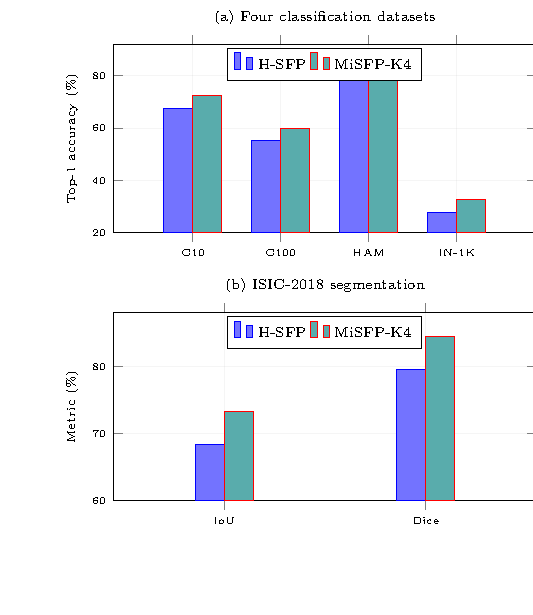
\includegraphics[width=\columnwidth]{figures/empirical_results.pdf}
\caption{Performance after 200 rounds: (a) IID top-1 accuracy on four classification datasets and (b) foreground IoU and Dice on ISIC-2018. Bars show means; SDs are reported in \cref{tab:classification200,tab:segmentation200}. Reference baseline protocols are distinguished from the matched study in the experimental setup.}
\label{fig:empirical}
\end{figure}

\subsection{Component Retention and Sensitivity}

\noindent\textbf{Across-source retention.} MiSFP-K1 has lower reported accuracy means than H-SFP in all three matched partitions (\cref{tab:main}). Retaining source components in MiSFP-Edge raises accuracy relative to K1 throughout: under IID, the mean increases from $54.93\%$ to $59.87\%$, while under Dir($\alpha=0.1$) it increases from $5.12\pm0.11\%$ to $6.82\pm0.06\%$. The results support retaining distinct source components before synthesis within the tested pipeline.

\noindent\textbf{Within-client components.} K2 and K4 provide additional gains over Edge under heterogeneous partitions. Under Dir($\alpha=0.1$), they reach $8.75\pm0.16\%$ and $9.46\pm0.31\%$, respectively, corresponding to gains of 1.93 and 2.64 points over Edge and 3.26 and 3.97 points over H-SFP. Under IID, their means remain close to Edge, indicating that across-source retention accounts for most of the observed improvement in that setting (Fig.~\ref{fig:diagnostics}(a)).
Moreover, local support also affects this comparison. With the default $s_{\min}=3$, a two-component fit requires at least six fitting features and a four-component fit requires at least twelve; clustering can impose further restrictions through the assignment counts. Changing the partition alters both class heterogeneity and local support. Consequently, the partition-dependent results cannot be attributed exclusively to differences in semantic multimodality, and requested component counts should not be interpreted as realized counts.

\noindent\textbf{Adaptive allocation.} Adaptive improves on H-SFP but remains below fixed K2 and K4 in all three partitions. Under Dir($\alpha=0.1$), it achieves $7.50\pm0.14\%$ accuracy, with an average of $1.66\pm0.03$ retained components per class, compared with $1.58\pm0.02$ for Edge. These retained counts reflect pooling and compression as well as local selection; they do not establish how often clients select $K>1$.
Under IID, Adaptive and Edge have identical reported accuracy and macro-F1 means and SDs. The tested selector therefore provides limited additional predictive benefit in that setting. We interpret Adaptive as a diagnostic allocation heuristic: its held-out density criterion does not directly optimize downstream prediction, and its results characterize the tested rule, thresholds, and support constraints. Fixed K2 and K4 provide the strongest results among the evaluated allocations.

\noindent\textbf{Minimum support and boundary sampling.} Under Dir($\alpha=0.1$), the minimum-support sweep changes accuracy from $7.23\pm0.26\%$ at support ten to $7.74\pm0.09\%$ at support one (Fig.~\ref{fig:diagnostics}(b)). Increasing the boundary-estimation count from ten to 200 samples per component changes accuracy from $7.44\pm0.07\%$ to $7.66\pm0.18\%$ (Fig.~\ref{fig:diagnostics}(c)). These endpoint differences are smaller than those associated with component retention in the matched study; they remain specific to the tested sweep configurations.

\begin{figure}[t]
\centering
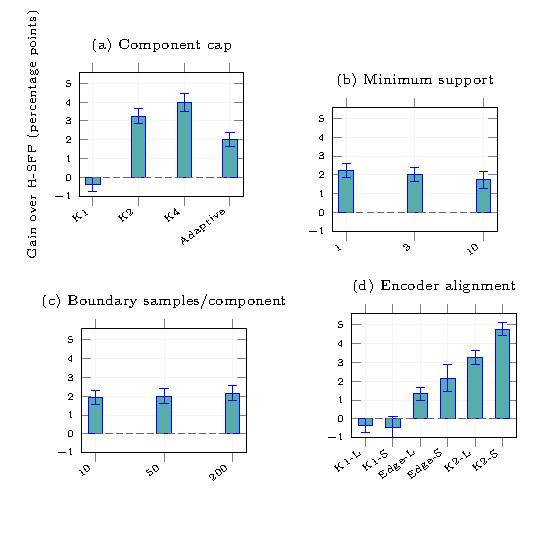
\includegraphics[width=\columnwidth]{figures/diagnostic_results.pdf}
\caption{Sensitivity and encoder-compatibility diagnostics after 200 rounds on CIFAR-100, Dir($\alpha=0.1$). Values are accuracy gains over the matched H-SFP mean of $5.49\%$. Error bars show $\sqrt{s_{\mathrm{method}}^2+s_{\mathrm{H\text{-}SFP}}^2}$ as descriptive dispersion, not paired-difference SDs or confidence intervals. Panels compare (a) component configurations, (b) minimum component support, (c) boundary Monte Carlo samples per component, and (d) local (L) and shared-snapshot (S) extraction.}
\label{fig:diagnostics}
\end{figure}

\subsection{Communication and Resource Costs}

\noindent\textbf{Communication breakdown.} \Cref{tab:resources} reports cumulative communication, runtime, and peak allocated memory under Dir($\alpha=0.1$). The analytical packet-body expression in \cref{eq:bytes} describes individual messages; the measured totals additionally include packet headers, repeated transmissions, and model synchronization.
Model synchronization contributes $4285.1\pm0.0$\,MiB to every listed configuration and dominates total traffic. K2 and K4 use $4724.7\pm2.4$\,MiB and $4776.8\pm3.7$\,MiB in total, compared with $4541.2\pm1.3$\,MiB for H-SFP, giving increases of approximately 4.0\% and 5.2\%.

The prototype-specific increases are substantially larger. Subtracting synchronization from the rounded H-SFP total gives approximately 256.1\,MiB of prototype traffic. K2 and K4 transmit 439.57 and 491.64\,MiB across the two boundaries, corresponding to increases of approximately 71.6\% and 92.0\%. Thus, the modest total-communication increments depend on the synchronization-dominated operating point. Both prototype traffic and total traffic are needed to assess the cost of retaining additional components.

\begin{table*}[t]
\caption{Communication and resource costs after 200 rounds on CIFAR-100, Dir($\alpha=0.1$): mean $\pm$ SD over three seeds. C--E and E--C denote client--edge and edge--cloud prototype traffic. Total communication includes $4285.1\pm0.0$\,MiB of model synchronization for every method. The boundary-specific prototype breakdown is unavailable for H-SFP. Measured packet sizes include headers, which are excluded from the body-size expression in \cref{eq:bytes}.}
\label{tab:resources}
\centering
\footnotesize
\setlength{\tabcolsep}{4pt}
\begin{tabular*}{\textwidth}{@{\extracolsep{\fill}}lccccc@{}}
\toprule
Method & C--E (MiB) & E--C (MiB) & Total (MiB) & Runtime (s) & Peak memory (MiB)\\
\midrule
H-SFP & n/a & n/a & $4541.2\pm1.3$ & $70398\pm1859$ & $2150\pm6$\\
MiSFP-K1 & $120.03\pm0.17$ & $142.06\pm1.42$ & $4547.2\pm1.4$ & $70579\pm1794$ & $2151\pm5$\\
MiSFP-Edge & $120.03\pm0.17$ & $235.65\pm0.33$ & $4640.8\pm0.5$ & $68828\pm169$ & $2150\pm5$\\
MiSFP-K2 & $150.90\pm0.75$ & $288.67\pm1.79$ & $4724.7\pm2.4$ & $68940\pm138$ & $2149\pm6$\\
MiSFP-K4 & $176.74\pm1.29$ & $314.90\pm2.72$ & $4776.8\pm3.7$ & $69208\pm295$ & $2151\pm5$\\
MiSFP-Adaptive & $127.92\pm0.15$ & $248.65\pm0.71$ & $4661.7\pm0.9$ & $70840\pm1656$ & $2151\pm5$\\
\bottomrule
\end{tabular*}
\end{table*}

\noindent\textbf{Packet-budget sensitivity.} Budget ratios are defined relative to the configured float32 K1 reference cap at each boundary. A float16 K2 configuration using the $1.0\times$ reference caps achieves $8.86\pm0.31\%$ accuracy with $4494.7\pm2.2$\,MiB total communication. Relative to matched H-SFP, this configuration gains 3.37 points while using approximately 1.0\% less total communication. Equal per-packet caps do not imply equal cumulative traffic because packet occupancy and retained component counts vary.
At $1.5\times$ and $2.0\times$ the reference cap, K2 reaches $8.48\pm0.24\%$ and $8.87\pm0.07\%$. Adaptive reaches $7.46\pm0.16\%$, $7.49\pm0.22\%$, and $7.32\pm0.22\%$ at $1.0\times$, $1.5\times$, and $2.0\times$, respectively. Across the tested configurations, larger caps are not associated with uniformly higher mean accuracy. The float16 matched setting jointly changes precision and component retention, so its result does not isolate either factor.

\noindent\textbf{Runtime and memory.} Mean runtimes range from 68828 to 70840 seconds, without a monotonic ordering by component count. Peak allocated GPU-memory means remain between 2149 and 2151\,MiB. These observations characterize the shared-GPU execution setting; they do not establish a runtime advantage, negligible incremental overhead, or per-client memory savings. The complexity analysis in \cref{sec:analysis} describes scaling, while isolated measurements of construction, merging, sampling, and boundary estimation are needed to quantify practical overhead.

\subsection{Representation Fidelity and Encoder Compatibility}

\noindent\textbf{Mixtures versus moment collapse.} \Cref{tab:fidelity} compares each K2 mixture with a single diagonal Gaussian derived from the same packet and matched to its unfloored diagonal moments. This controls the source packet while examining the effect of retaining multiple components.
Mixtures have lower mean SWD and MMD under both extraction regimes. Local-extraction MMD decreases from $0.1368\pm0.0151$ to $0.1221\pm0.0141$, while shared-snapshot MMD decreases from $0.0664\pm0.0016$ to $0.0530\pm0.0012$. In contrast, mixture NLL is higher in both regimes and varies substantially across seeds. Negative NLL values are valid for continuous densities.

These results support a metric-dependent interpretation: retaining components reduces the reported sample-based discrepancies but does not improve held-out likelihood. The comparison evaluates component retention within the diagonal-covariance interface; it does not establish superiority over richer covariance models. SWD and MMD also do not numerically evaluate the conditional loss bound in \cref{sec:analysis}.

\begin{table*}[t]
\caption{Representation fidelity and encoder compatibility on held-out real features after 200 rounds: mean $\pm$ SD over three seeds. Lower NLL, SWD, and MMD are better. The between-source ratio is computed from real features and is shared by both representations within each extraction regime.}
\label{tab:fidelity}
\centering
\footnotesize
\setlength{\tabcolsep}{4pt}
\begin{tabular*}{\textwidth}{@{\extracolsep{\fill}}llcccc@{}}
\toprule
Extraction & Representation & NLL (nat/dim) & SWD & MMD & Between-source ratio\\
\midrule
Local & Single Gaussian (collapsed K2 packet) & $-0.867\pm0.037$ & $0.053\pm0.004$ & $0.1368\pm0.0151$ & $0.474\pm0.049$\\
Local & MiSFP-K2 mixture & $-0.312\pm0.339$ & $0.051\pm0.005$ & $0.1221\pm0.0141$ & $0.474\pm0.049$\\
Shared snapshot & Single Gaussian (collapsed K2 packet) & $-0.970\pm0.050$ & $0.033\pm0.001$ & $0.0664\pm0.0016$ & $0.346\pm0.078$\\
Shared snapshot & MiSFP-K2 mixture & $-0.429\pm0.407$ & $0.031\pm0.001$ & $0.0530\pm0.0012$ & $0.346\pm0.078$\\
\bottomrule
\end{tabular*}
\end{table*}

\noindent\textbf{Shared encoder snapshot.} Local extraction uses each client's updated encoder, whereas shared-snapshot extraction uses a common encoder checkpoint. Fig.~\ref{fig:diagnostics}(d) compares these regimes for K1, Edge, and K2. The between-source dispersion ratio decreases from $0.474\pm0.049$ to $0.346\pm0.078$. This is consistent with encoder differences contributing to source separation, but dispersion alone cannot determine whether an individual component represents a semantic subpopulation.

With shared-snapshot extraction, K2 accuracy increases from $8.75\pm0.16\%$ to $10.26\pm0.05\%$. K1 changes little, reaching $5.04\pm0.47\%$ compared with $5.12\pm0.11\%$ under local extraction. K2 therefore retains a positive accuracy difference over K1 in both regimes. This supports the utility of retaining components under both extraction settings without identifying the semantic origin of the retained structure.

The intervention changes the encoder checkpoint as well as coordinate comparability, and a common client encoder does not guarantee alignment of independently trained edge-output mappings. It also raises total communication to $15060.3\pm2.5$\,MiB, approximately $3.19$ times the local-extraction K2 total of $4724.7\pm2.4$\,MiB. The shared-snapshot result is therefore interpreted as a sensitivity analysis with additional communication cost.
\section{Discussion and Limitations}
\label{sec:discussion}

\noindent\textbf{Practical implications.}~The CIFAR-100 results support retaining separate source components before synthesis, with additional local components improving prediction under the tested non-IID partitions (\cref{sec:experiments}). Partitioning also changes local class support, so these differences cannot be attributed exclusively to heterogeneity. Component allocation should be assessed jointly with support, coordinate compatibility, and communication. The modest increases in total traffic occur in a synchronization-dominated configuration; the larger prototype-specific increases remain relevant when synchronization is less frequent. Mixed fidelity results further motivate evaluating predictive utility alongside several distributional criteria.

\noindent\textbf{Representation and selection.}~Diagonal covariance keeps component storage and transmission linear in feature dimension, whereas full covariance requires quadratic storage. Differences between component means can still represent class-level dependence, although each component omits internal correlations. The experiments do not establish that diagonal mixtures are preferable to richer covariance models under equal byte budgets. Limited support can also destabilize variance estimates and component selection. K-means minimizes squared distances, while the adaptive rule evaluates held-out likelihood; neither directly optimizes downstream prediction. Fixed K2 and K4 provide the strongest predictive results among the allocations. Adaptive one is interpreted as an evaluated density-based heuristic whose performance depends on its criterion, thresholds, and eligible support. Post-compression counts cannot establish local selection frequencies.

\noindent\textbf{Encoder compatibility.}~Matching packet metadata and periodic synchronization establish structural compatibility without guaranteeing semantic coordinate alignment. Retained components can represent population structure, encoder differences, or both. Shared-snapshot results demonstrate sensitivity to the extraction regime, but the intervention changes the encoder checkpoint and communication cost, preventing attribution of the improvement solely to alignment. Between-source dispersion cannot identify the semantic origin of individual components, and a common client encoder does not itself align independently trained edge-output mappings.

\noindent\textbf{Approximation guarantees.}~The merge operator preserves class mass, means, and coordinate-wise second moments in exact arithmetic (\cref{sec:analysis}). These identities leave higher-order structure unconstrained: merging can absorb low-mass components and alter density valleys or predictions. The greedy score provides a deterministic reduction rule without guaranteeing globally optimal compression. Boundary re-estimation adds finite-sample and diagonal-approximation errors, while serialization introduces quantization error. The conditional loss bounds describe fixed-predictor sensitivity under explicit assumptions; they do not establish convergence or monotonic improvement with component count.

\noindent\textbf{Privacy.}~Keeping raw examples local does not itself provide a formal privacy guarantee. Counts, moments, and small-support components can expose information about contributing data. The minimum-support rule constrains multi-component fitting and permits a single-component fallback; it is not a privacy reporting threshold. Privacy protection requires an explicit threat model and additional mechanisms, such as suitable reporting policies, differential privacy, or secure aggregation, together with attack evaluation and measurement of the resulting utility and communication tradeoffs.

\noindent\textbf{Empirical scope.}~The findings concern the tested datasets, architectures, and split configurations. The low absolute accuracy under severe heterogeneity limits deployment claims despite the improvement over H-SFP. Focused ablations use five edges and three seeds, whereas reference benchmarks use ten edges and five runs; these run sets are not pooled. Three seeds provide a limited assessment of variability, and shared-GPU measurements do not establish comparative runtime efficiency or per-client memory savings. Further evaluation should prioritize controlled overhead measurements, alternative compression and covariance choices, and additional model families, split locations, and client populations.
\section{Conclusion}
\label{sec:conclusion}

This paper presents \method{}, a statistical feature-transfer framework for hierarchical split federated learning. MiSFP combines support-weighted diagonal Gaussian mixtures, output-space re-estimation after the nonlinear edge segment, and deterministic class-preserving compression under component caps and optional boundary-specific byte budgets. The analysis establishes exact mass and diagonal-moment preservation, a per-merge transport bound, packet and computational costs, and conditional fixed-predictor loss bounds. Evaluation covers four classification datasets and ISIC-2018 segmentation, with matched CIFAR-100 ablations supporting the utility of component retention. Under Dir($\alpha=0.1$), MiSFP-K4 improves accuracy over H-SFP by 3.97 percentage points, with approximately 5.2\% more total communication and 92\% more prototype traffic. The low absolute accuracy under severe heterogeneity, metric-dependent fidelity results, and sensitivity to encoder extraction limit broader deployment claims. These findings support evaluating predictive utility together with representation quality, coordinate compatibility, and both prototype and synchronization costs. Future work should investigate utility-aware component allocation, coordinate alignment, controlled overhead measurements, and privacy protection for communicated summaries.
\appendices
% \section{Implementation and Reproducibility Details}\label{app:repro}
\subsection{Packet semantics}
Packets use magic bytes \texttt{MSFP}; a JSON header stores feature-space metadata, source, round, and precision. Each class record stores int32 class id and component count. Each component stores int32 local id, float32 mass, and two length-$d$ moment vectors in float16 or float32. Internally, fitting and pooling use float64. Serialization/de-serialization is executed in the training path so the receiver observes quantization. Component ids are reassigned after canonical ordering and never establish identity across clients.

\subsection{Default controls}
Defaults are $s_{\min}=3$, three k-means initializations, 50 Lloyd iterations, center reservoir 4096, adaptive cap four, validation fraction 0.3, minimum four validation samples, and improvement threshold 0.02 nat/dimension. The NLL variance floor is $\max(10^{-6},0.01\bar v_c)$ and the sampling floor is $10^{-12}$. Propagate mode uses 50 transformation samples per component; refit mode uses 200 per class. These values describe code defaults, not optimized choices.

% \subsection{Proof detail for \cref{prop:moments}}
% For scalar coordinate $j$, let $s_x=v_x+\mu_x^2$. Expanding the numerator of \cref{eq:poolvar} gives
% \begin{align*}
% m(v+\mu^2)&=a v_a+b v_b+a(\mu_a-\mu)^2\\
% &\quad+b(\mu_b-\mu)^2+m\mu^2\\
% &=a(v_a+\mu_a^2)+b(v_b+\mu_b^2)\\
% &\quad-2\mu(a\mu_a+b\mu_b)+2m\mu^2\\
% &=a s_a+b s_b.
% \end{align*}
% The vector result follows coordinate-wise. Floating-point serialization can perturb this algebra, which is why empirical audits compare both pre-wire float64 and received values.


% \section*{Acknowledgment}
% This work was supported by the Green Serverless Computing for Resource-Efficient AI Training Project at VinUniversity under Grant VUNI.CEI.FS\_0002.
\bibliographystyle{IEEEtran}
\bibliography{main}
\end{document}
